%%%%%%%%%%%%%%%%%%%%%%%%%%%%%%%%%%%%%%%%%%%%%%%%%%%%%%%%%%%%%%%%%%%%%%%%%%%%%%%
%                       CARGA DE LA CLASE DE DOCUMENTO                        %
%                                                                             %
% Las opciones admisibles son:                                                %
%      12pt / 11pt            (tamaño del cuerpo de letra; no usar 10pt)      %
%                                                                             %
% catalan/spanish/english     (idioma principal del trabajo)                  %
%                                                                             % 
% french/italian/german...    (si necesitáis usar otro idioma adicional)      %
%                                                                             %
% listoffigures               (El documento incluye un Índice de figuras)     %
% listoftables                (El documento incluye un Índice de tablas)      %
% listofquadres               (El documento incluye un Índice de cuadros)     %
% listofalgorithms            (El documento incluye un Índice de algoritmos)  %
%                                                                             %
%%%%%%%%%%%%%%%%%%%%%%%%%%%%%%%%%%%%%%%%%%%%%%%%%%%%%%%%%%%%%%%%%%%%%%%%%%%%%%%

\documentclass[11pt,spanish,listoffigures,listoftables]{tfgetsinf}

%%%%%%%%%%%%%%%%%%%%%%%%%%%%%%%%%%%%%%%%%%%%%%%%%%%%%%%%%%%%%%%%%%%%%%%%%%%%%%%
%                     CODIFICACIÓN DEL ARCHIVO FUENTE                         %
%                                                                             %
%    Windows suele usar 'ansinew'                                             %
%    en Linux es posible que sea 'latin1' o 'latin9'                          %
%    Pero lo más recomendable es usar utf8 (unicode 8)                        %
%                                          (si vuestro editor lo permite)     % 
%%%%%%%%%%%%%%%%%%%%%%%%%%%%%%%%%%%%%%%%%%%%%%%%%%%%%%%%%%%%%%%%%%%%%%%%%%%%%%%

\usepackage[utf8]{inputenc} 


%%%%%%%%%%%%%%%%%%%%%%%%%%%%%%%%%%%%%%%%%%%%%%%%%%%%%%%%%%%%%%%%%%%%%%%%%%%%%%%
%                       OTROS PAQUETES Y DEFINICIONES                         %
%                                                                             %
%%%%%%%%%%%%%%%%%%%%%%%%%%%%%%%%%%%%%%%%%%%%%%%%%%%%%%%%%%%%%%%%%%%%%%%%%%%%%%%

\usepackage{glossaries}
\usepackage{textcomp}
\usepackage{booktabs}
\usepackage{float}
\usepackage{enumitem}
\usepackage{graphicx}
\usepackage{subcaption}
\usepackage{tabularx}
\usepackage{pgfplots}
\pgfplotsset{compat=1.18}

% Listings para código
\usepackage{listings}
\lstset{
  basicstyle=\ttfamily\small,
  frame=single,
  breaklines=true,
  postbreak=\mbox{\textcolor{gray}{$\hookrightarrow$}\space},
  columns=fullflexible,
  keepspaces=true,
  numbers=none
}

% Bibliografía
\usepackage[backend=biber,style=numeric,sorting=none]{biblatex}
\addbibresource{bibliografia.bib}

% Hyperref siempre al final
\usepackage{hyperref}
\hypersetup{
  colorlinks=true,
  linkcolor=black,
  urlcolor=cyan,
  citecolor=black
}
%%%%%%%%%%%%%%%%%%%%%%%%%%%%%%%%%%%%%%%%%%%%%%%%%%%%%%%%%%%%%%%%%%%%%%%%%%%%%%%
%                          DATOS DEL TRABAJO                                  %
%                                                                             %
% título alumno, titor y curso académico                                      %
%%%%%%%%%%%%%%%%%%%%%%%%%%%%%%%%%%%%%%%%%%%%%%%%%%%%%%%%%%%%%%%%%%%%%%%%%%%%%%%

\title{Plantilla proyectos \\ Latex para proyectos extensos, trabajos y tesis}
\author{Miquel Gómez}
% \tutor{No}
% \curs{MUIARFID}

%%%%%%%%%%%%%%%%%%%%%%%%%%%%%%%%%%%%%%%%%%%%%%%%%%%%%%%%%%%%%%%%%%%%%%%%%%%%%%%
%                     PARAULES CLAU/PALABRAS CLAVE/KEY WORDS                  %
%                                                                             %
% Independentment de la llengua del treball, s'hi han d'incloure              %
% les paraules clau i el resum en els tres idiomes                            %
%%%%%%%%%%%%%%%%%%%%%%%%%%%%%%%%%%%%%%%%%%%%%%%%%%%%%%%%%%%%%%%%%%%%%%%%%%%%%%%

\keywords{
    Clasificaciò de texts. 
} % Paraules clau 
{
   Clasificación de textos; Películas; Transformers; LLMs; Machine Learning
} % Palabras clave
{
    Text clasification.
} % Key words


%%%%%%%%%%%%%%%%%%%%%%%%%%%%%%%%%%%%%%%%%%%%%%%%%%%%%%%%%%%%%%%%%%%%%%%%%%%%%%%
%                                                                             %
%                              INICI DEL DOCUMENT                             %
%                                                                             %
%%%%%%%%%%%%%%%%%%%%%%%%%%%%%%%%%%%%%%%%%%%%%%%%%%%%%%%%%%%%%%%%%%%%%%%%%%%%%%%

\begin{document} 


%%%%%%%%%%%%%%%%%%%%%%%%%%%%%%%%%%%%%%%%%%%%%%%%%%%%%%%%%%%%%%%%%%%%%%%%%%%%%%%
%              RESUMENES DEL TFG EN VALENCIA, CASTELLA I ANGLES               %
%%%%%%%%%%%%%%%%%%%%%%%%%%%%%%%%%%%%%%%%%%%%%%%%%%%%%%%%%%%%%%%%%%%%%%%%%%%%%%%


\begin{abstract}[spanish]

\end{abstract}

%%%%%%%%%%%%%%%%%%%%%%%%%%%%%%%%%%%%%%%%%%%%%%%%%%%%%%%%%%%%%%%%%%%%%%%%%%%%%%%
%                                                                             %
%                              CONTENIDO DEL TREBAJO                          %
%                                                                             %
%%%%%%%%%%%%%%%%%%%%%%%%%%%%%%%%%%%%%%%%%%%%%%%%%%%%%%%%%%%%%%%%%%%%%%%%%%%%%%%

%%%%%%%%%%%%%%%%%%%%%%%%%%%%%%%%%%%%%%%%%%%%%%%%%%%%%%%%%%%%%%%%%%%%%%%%%%%%%%%
%                                  ÍDNICE                                     %
%%%%%%%%%%%%%%%%%%%%%%%%%%%%%%%%%%%%%%%%%%%%%%%%%%%%%%%%%%%%%%%%%%%%%%%%%%%%%%%
\clearpage
\tableofcontents
% \listoffigures
% \listoftables

%%%%%%%%%%%%%%%%%%%%%%%%%%%%%%%%%%%%%%%%%%%%%%%%%%%%%%%%%%%%%%%%%%%%%%%%%%%%%%%
%                                GLOSARIO                                     %
%%%%%%%%%%%%%%%%%%%%%%%%%%%%%%%%%%%%%%%%%%%%%%%%%%%%%%%%%%%%%%%%%%%%%%%%%%%%%%%
% \glsaddall
% \printglossaries
% \printnoidxglossaries


%%%%%%%%%%%%%%%%%%%%%%%%%%%%%%%%%%%%%%%%%%%%%%%%%%%%%%%%%%%%%%%%%%%%%%%%%%%%%%%
%                                  INTRODUCCION                               %
%%%%%%%%%%%%%%%%%%%%%%%%%%%%%%%%%%%%%%%%%%%%%%%%%%%%%%%%%%%%%%%%%%%%%%%%%%%%%%%
\chapter{Introducción}

\begin{lstlisting}[language=Python, basicstyle=\ttfamily\small, frame=single, numbers=left, breaklines=true]
def generate_prompt(df_train: pd.DataFrame, df_batch: pd.DataFrame, genres: str) -> str:
    prompt = f"""
    Classify the following movie in any of these genres. More than one genre can be assigned.
    Genres: {genres}

    ==============================================
    """

    for _, row in df_train.iterrows():
        prompt += f"Movie title: {row['movie_name']}\n"
        prompt += f"Plot: {row['description']}\n"
        prompt += f"Actual genres: {row['genre']}\n"
        prompt += "-------------------\n"

    prompt += """
    ==============================================
    Now, classify the following movies returning a structured JSON
    response with the movie names and their genres.
    """

    for _, row in df_batch.iterrows():
        prompt += f"Movie title: {row['movie_name']}\n"
        prompt += f"Plot: {row['description']}\n\n"

    return prompt
\end{lstlisting}


%%%%%%%%%%%%%%%%%%%%%%%%%%%%%%%%%%%%%%%%%%%%%%%%%%%%%%%%%%%%%%%%%%%%%%%%%%%%%
%                         ANÁLISIS DEL PROBLEMA                               %
%%%%%%%%%%%%%%%%%%%%%%%%%%%%%%%%%%%%%%%%%%%%%%%%%%%%%%%%%%%%%%%%%%%%%%%%%%%%%%%
\mainmatter
\chapter{Codificación}
Lore ipsum dolor sit amet, consectetur adipiscing elit. Sed non risus. Suspendisse lectus tortor, dignissim sit amet, adipiscing nec, ultricies sed, dolor. Cras elementum ultrices diam. Maecenas ligula massa, varius a, semper congue, euismod non, mi. Proin porttitor, orci nec nonummy molestie, enim est eleifend mi, non fermentum diam nisl sit amet erat. Duis semper. Duis arcu massa, scelerisque vitae, consequat in, pretium a, enim. Pellentesque congue. Ut in risus volutpat libero pharetra tempor. Cras vestibulum bibendum augue. Praesent egestas leo in pede. Praesent blandit odio eu enim. Pellentesque sed dui ut augue blandit sodales. Vestibulum ante ipsum primis in faucibus orci luctus et ultrices posuere cubilia Curae; Aliquam nibh. Mauris ac mauris sed pede pellentesque fermentum. Maecenas adipiscing ante non diam sodales hendrerit.
\section{Tecnologías}

\subsection{Modelos clásicos}
Example text for the section on classical models. This section will cover traditional machine learning algorithms and their applications in text classification.

\subsection{Transformers}
More example text for the section on transformers. This section will discuss the architecture of transformer models, their advantages, and how they have revolutionized natural language processing tasks.

\subsection{LLMs (Grandes Modelos de lenguaje)}

\section{Dataset}


\section{Manejo del dataset}

\subsection{Procesado del dataset}

\section{Evaluación}

%%%%%%%%%%%%%%%%%%%%%%%%%%%%%%%%%%%%%%%%%%%%%%%%%%%%%%%%%%%%%%%%%%%%%%%%%%%%%%%
%                           TÉCNOLOGÍAS PLANTEADAS                            %
%%%%%%%%%%%%%%%%%%%%%%%%%%%%%%%%%%%%%%%%%%%%%%%%%%%%%%%%%%%%%%%%%%%%%%%%%%%%%%%
\chapter{Implementación}


%%%%%%%%%%%%%%%%%%%%%%%%%%%%%%%%%%%%%%%%%%%%%%%%%%%%%%%%%%%%%%%%%%%%%%%%
\section{Modelos clásicos}

\section{Transformers}

\section{LLMs}


%%%%%%%%%%%%%%%%%%%%%%%%%%%%%%%%%%%%%%%%%%%%%%%%%%%%%%%%%%%%%%%%%%%%%%%%%%%%%%%
%                               RESULTADOS DE LA SOLUCIón                     %
%%%%%%%%%%%%%%%%%%%%%%%%%%%%%%%%%%%%%%%%%%%%%%%%%%%%%%%%%%%%%%%%%%%%%%%%%%%%%%%
\chapter{Resultado de las soluciones}
A continuación presentamos los resultados que han obtenido los modelos planteados en cada categoría.

\section{Clásicos}

\section{Transformers}


\section{LLMs}


\section{Resumen resultados}
A continuación se muestran los resultados WER obtenidos en los diferentes ejercicios realizados:

\begin{figure}[H]
\centering
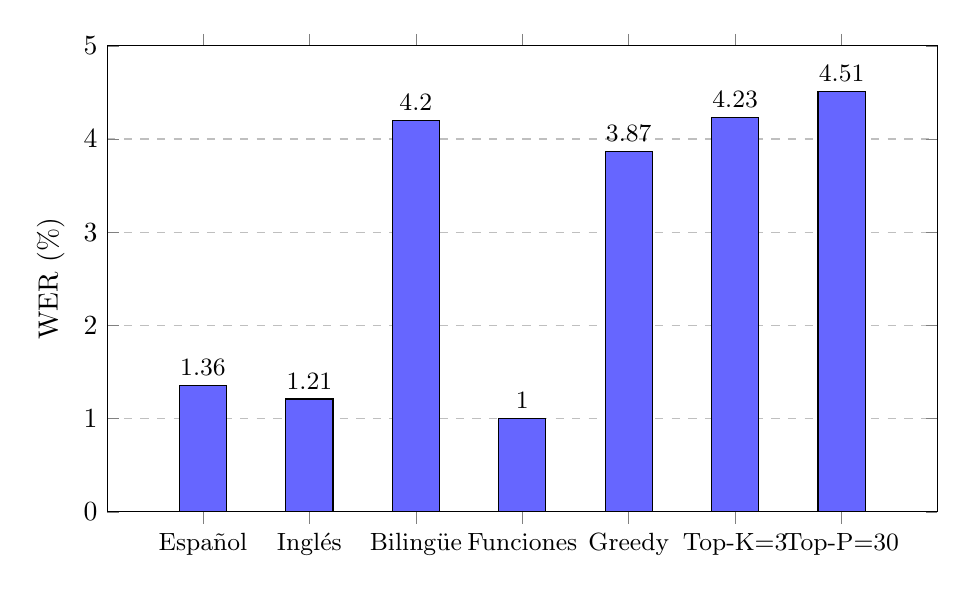
\begin{tikzpicture}
\begin{axis}[
    ybar,
    bar width=0.6cm,
    width=\textwidth,
    height=7.5cm,
    ylabel={WER (\%)},
    symbolic x coords={Español, Inglés, Bilingüe, Funciones, Greedy, Top-K=3, Top-P=30},
    xtick=data,
    x tick label style={font=\small},
    ymin=0,
    ymax=5,
    ymajorgrids=true,
    grid style=dashed,
    enlarge x limits=0.15,
    nodes near coords,
    nodes near coords align={vertical},
    every node near coord/.append style={font=\small},
]

% WER scores
\addplot[fill=blue!60] coordinates {
    (Español, 1.36)
    (Inglés, 1.21)
    (Bilingüe, 4.20)
    (Funciones, 1.0)
    (Greedy, 3.87)
    (Top-K=3, 4.23)
    (Top-P=30, 4.51)
};

\end{axis}
\end{tikzpicture}
\caption{Comparación de WER obtenido en cada ejercicio. Español e Inglés corresponden al Ejercicio 1, Bilingüe al Ejercicio 2, Funciones al Ejercicio 3, y Greedy Extra al ejercicio extra con decodificación greedy.}
\label{fig:resultados_finales}
\end{figure}

%%%%%%%%%%%%%%%%%%%%%%%%%%%%%%%%%%%%%%%%%%%%%%%%%%%%%%%%%%%%%%%%%%%%%%%%%%%%%%%
%                                 CONCLUSIONES                                 %
%%%%%%%%%%%%%%%%%%%%%%%%%%%%%%%%%%%%%%%%%%%%%%%%%%%%%%%%%%%%%%%%%%%%%%%%%%%%%%%
\chapter{Conclusiones}

%%%%%%%%%%%%%%%%%%%%%%%%%%%%%%%%%%%%%%%%%%%%%%%%%%%%%%%%%%%%%%%%%%%%%%%%%%%%%%%
%                                                                             %
%                                BIBLIOGRAFIA                                 %
%                                                                             %
%%%%%%%%%%%%%%%%%%%%%%%%%%%%%%%%%%%%%%%%%%%%%%%%%%%%%%%%%%%%%%%%%%%%%%%%%%%%%%%
\cleardoublepage
\printbibliography

%%%%%%%%%%%%%%%%%%%%%%%%%%%%%%%%%%%%%%%%%%%%%%%%%%%%%%%%%%%%%%%%%%%%%%%%%%%%%%%
%                                                                             %
%                                 APÉNDICESS                                  %
%                                                                             %
%%%%%%%%%%%%%%%%%%%%%%%%%%%%%%%%%%%%%%%%%%%%%%%%%%%%%%%%%%%%%%%%%%%%%%%%%%%%%%%

% \APPENDIX
%%%%%%%%%%%%%%%%%%%%%%%%%%%%%%%%%%%%%%%%%%%%%%%%%%%%%%%%%%%%%%%%%%%%%%%%%%%%%%%
%                        EJEMPLOS DE CADA TIPO DE FACTURA                     %
%%%%%%%%%%%%%%%%%%%%%%%%%%%%%%%%%%%%%%%%%%%%%%%%%%%%%%%%%%%%%%%%%%%%%%%%%%%%%%%

% \chapter{Apéndice ejemplo}
% \label{appendix:ejemplos}


%%%%%%%%%%%%%%%%%%%%%%%%%%%%%%%%%%%%%%%%%%%%%%%%%%%%%%%%%%%%%%%%%%%%%%%%%%%%%%%
%                              FIN DEL DOCUMENTO                              %
%%%%%%%%%%%%%%%%%%%%%%%%%%%%%%%%%%%%%%%%%%%%%%%%%%%%%%%%%%%%%%%%%%%%%%%%%%%%%%%
\end{document}
